% definitions.tex
\usepackage{tcolorbox}
\usepackage{tikz}
\usetikzlibrary{positioning, arrows.meta, shapes.geometric}

% Define custom environments
\newenvironment{mathmodel}{
    \begin{tcolorbox}[colback=violet!5, colframe=white, sharp corners, boxrule=0pt, title=Mathematical Model]
}{
    \end{tcolorbox}
}

\newenvironment{mathmod}{
    \begin{tcolorbox}[colback=blue!5, colframe=white, sharp corners, boxrule=0pt, title=Mathematical Model]
}{
    \end{tcolorbox}
}

\newenvironment{codebox}{
    \begin{tcolorbox}[colback=gray!10, colframe=black, sharp corners, boxrule=0.5pt, title=Code Box]
}{
    \end{tcolorbox}
}

% Define custom figure commands
\def\imgInDelphiRelation#1{
    \refstepcounter{figure} % Increment figure counter
    \newline
    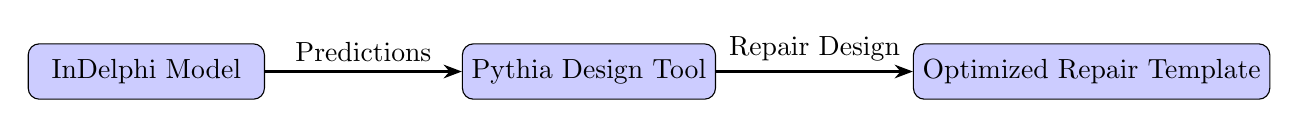
\begin{tikzpicture}[
        node distance=2.5cm,
        process/.style={rectangle, draw, fill=blue!20, rounded corners, text centered, minimum height=2em, minimum width=3cm},
        arrow/.style={thick, ->, >=Stealth}
    ]
    \node[process] (indelphi) {InDelphi Model};
    \node[process, right=of indelphi] (pythia) {Pythia Design Tool};
    \node[process, right=of pythia] (template) {Optimized Repair Template};

    \draw[arrow] (indelphi) -- node[anchor=south] {Predictions} (pythia);
    \draw[arrow] (pythia) -- node[anchor=south] {Repair Design} (template);
    \end{tikzpicture}
    \newline
    \noindent\parbox[t]{0.48\textwidth}{\textbf{Figure \thefigure}: #1}\\[1em]
}

\def\imgInDelphiLearning#1{
    \refstepcounter{figure} % Increment figure counter
    \newline
    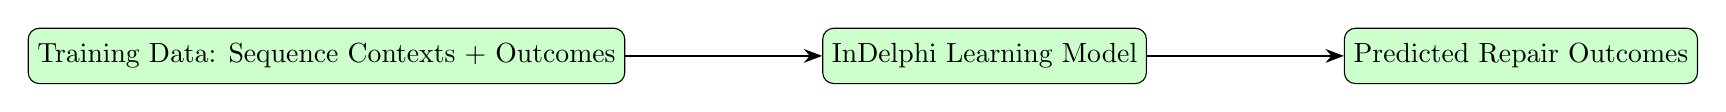
\begin{tikzpicture}[
        node distance=2.5cm,
        process/.style={rectangle, draw, fill=green!20, rounded corners, text centered, minimum height=2em, minimum width=3cm},
        arrow/.style={thick, ->, >=Stealth}
    ]
    \node[process] (input) {Training Data: Sequence Contexts + Outcomes};
    \node[process, right=of input] (model) {InDelphi Learning Model};
    \node[process, right=of model] (output) {Predicted Repair Outcomes};

    \draw[arrow] (input) -- (model);
    \draw[arrow] (model) -- (output);
    \end{tikzpicture}
    \newline
    \noindent\parbox[t]{0.48\textwidth}{\textbf{Figure \thefigure}: #1}\\[1em]
}

\def\imgMMEJDiagram#1{
    \refstepcounter{figure} % Increment figure counter
    \newline
    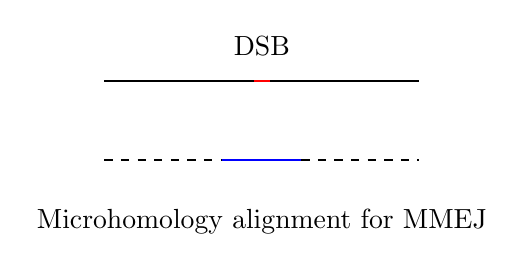
\begin{tikzpicture}
        \draw[thick] (0,0) -- (4,0); % DNA strand before cut
        \draw[thick, red] (1.9, 0) -- (2.1, 0); % Cut site
        \node[above] at (2,0.2) {DSB};

        % Microhomology alignment
        \draw[thick, dashed] (0, -1) -- (1.5, -1); % Left side alignment
        \draw[thick, dashed] (2.5, -1) -- (4, -1); % Right side alignment
        \draw[thick, blue] (1.5, -1) -- (2.5, -1); % Microhomology bridging

        \node[below] at (2, -1.5) {Microhomology alignment for MMEJ};
    \end{tikzpicture}
    \newline
    \noindent\parbox[t]{0.48\textwidth}{\textbf{Figure \thefigure}: #1}\\[1em]
}

\def\imgPythiaTemplate#1{
    \refstepcounter{figure} % Increment figure counter
    \newline
    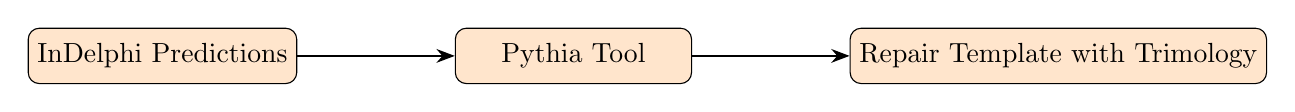
\begin{tikzpicture}[
        node distance=2cm,
        process/.style={rectangle, draw, fill=orange!20, rounded corners, text centered, minimum height=2em, minimum width=3cm},
        arrow/.style={thick, ->, >=Stealth}
    ]
    \node[process] (indelphi) {InDelphi Predictions};
    \node[process, right=of indelphi] (pythia) {Pythia Tool};
    \node[process, right=of pythia] (template) {Repair Template with Trimology};

    \draw[arrow] (indelphi) -- (pythia);
    \draw[arrow] (pythia) -- (template);
    \end{tikzpicture}
    \newline
    \noindent\parbox[t]{0.48\textwidth}{\textbf{Figure \thefigure}: #1}\\[1em]
}
